\section{Chapter 1}

\textbf{Energy transitions} are socio-technical processes that reshape the
nature or patterns of use of energy resources and/or technologies.

\textbf{A socio-ecological system} describes human and Earth-system
interactions as dynamic, interconnected, and co-produced by nature and society.

International frameworks to evaluate and manage social and environmental
challenges:

\begin{itemize}
	\item Convention of International Trade in Endangered Sepecies (CITES)
	\item Intergovernmental Panel on Climate Change (IPCC)
	\item Montreal Protocol to protect the ozone layer
	\item Agenda 21
	\item Sustainable Development Goals (SDG)
\end{itemize}

In the 70s, the concept of energy transition mostly referred to providing
energy access to poor communities to increase their quality of life. It was
also used then to refer to the growing need for coal resources in southwest
USA. Today, the phrase \textit{energy transition} refers to the move towards
low-carbon economy.

Holocene - current geological epoch, refers to the last 12000 years. Contenders
for the start of anthropocene epoch include the first major imprints on the
atmosphere from fossil fuels -- emissions of methande and carbon dioxide.
Another candidate is the date that marks the start of atmospheric nuclear
testing in early 50s.

International Energy Agency (IEA) (2010) suggests power demand will increase
from 18 trillion watts in 2020 to somewhere between 25 and 30 trillion watts by
2050. 

Starting in 2015,the world started to build more renewable energy than energy
infrastructure to burn fossil energy.

\textbf{Projections} are trends taken into the future based on some existing
trends or some BAU\footnote{business as usual} scenario.

\textbf{Forecasts} are made by taking these projections and modifying them with
assumptions about the future, such as new technologies or different rates of
change.

\textbf{Primary energy sources} are the natural resources taken from the earth:
coal, "wet" natural gas (wet because it contains water, methane, ethane, and
other gases), petroleum, solar and wind power, uranium, and other direct
sources of energy harvested.

\textbf{Final fuel products} and \textbf{energy carriers} are the energy
sources that directly provide energy services.

Example final fuels: gasoline, "dry" natural gas (dry because it mostly
contains methane), wood for a stove or campfire, hydrogen and electricty.

Example energy carriers: electricity, hydrogen, steam.

\textbf{Corporate Social Responsibility (CSR)} is an approach to sustainability
that focuses on encouraging the private sector through voluntary standards,
industry benchmarks to favour sustainable solutions under the pressure from
investors and social and reputational pressure.

\textbf{Wind, Water and Sunlight (WWS)} strategies focus on replacing current
energy systems with one run solely on electrification and renewables.

\textbf{Hard} and \textbf{soft} paths in energy transitions. Hard path refers
to coal and nuclear power, while soft is led by renewables and appropriate
technologies.

Aces of debates in energy transitions:

\begin{itemize}
	\item apolitical
	\item democratic
	\item command and control
	\item global
	\item centralized
	\item private
	\item clean
	\item political
	\item technocratic
	\item market
	\item local
	\item decentralized
	\item public
	\item renewable
\end{itemize}

\textit{
Political scientist Langdon Winner argued that some forms of energy production
like nuclear energy rely on authoritarian forms of social organization to
protect nuclear fuel and waste (Winner 1989). Uranium in the supply chain for
nuclear fuel and plutonium in the waste (or some fuels) require militarization
and heavy security as nuclear power plants because of vulnerability to
meltdown accidents or occasional releases of low-level radiation. Winner argues
that technologies are not neutral but can have inherent politics.
}

\textbf{Rebound efect} -- when energy savings resulting from savings behaviour
are just spent elsewhere on energy consuming activities. A classic example
from this perspective is a driver who substitutes a vehicle with a
fuel-efficient version, only to reap the benefits of its lower operating
expenses to commute longer and more frequently.

2000-watt society is a notion for balancing basic human needs with
overconsumption. 2000-watt of power is about 48 kWh energy per day.

Energy demand globally is still increasing.

World population in 1990 was 5.3 billion and annual elctricity consumption
per person 2.07 MWh per person. By 2015, population was 5.3 billion and energy
consumption 3.05 MWh.

China:
\begin{itemize}
	\item 19\% of world's population
	\item in 2013, 50\% of world's coal consumption was China
	\item leads in wind power
	\item added a lot of solar (for 3 consecutive years added more then US
	in total through all years)
\end{itemize}

Giorgios Kallis is the leading thinker and writer on the question of de-growth.
Degrowth thinkers look for steady-state energy systems and economies instead
of fixating on increasing GDP.

\textit{
Entropy laws mean that conversions of energy result in less useful work
available with each conversion. This is why the laws of thermodynamics dictate
that the end of the universe will be a cosmic heat death. The total amount of
energy will be the same as it always has, but none of it will be available to
do work.
}

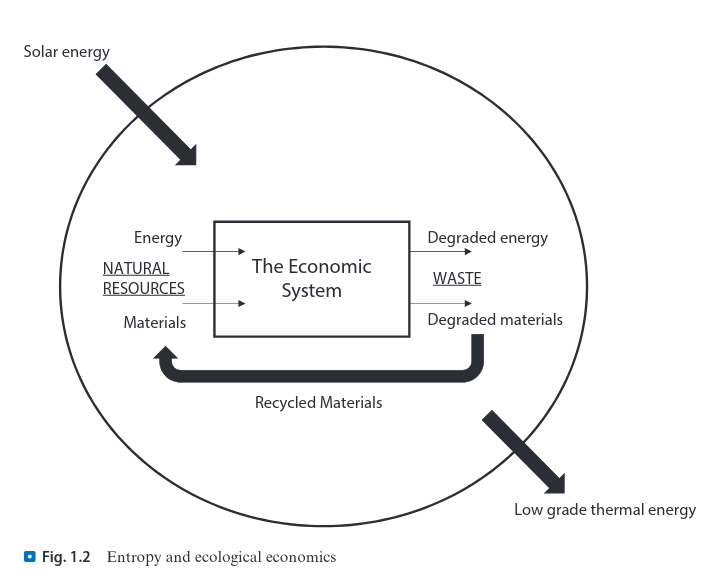
\includegraphics[scale=0.5]{content/img/entropy.png}

Eco-pragmatists argue in \textit{The Eco-modernist manifesto} that the nuclear
power is the only low-carbon energy technology capable of fully meeting the
urgent response needed to climate change.

Wind, water, solar (WWS) strategy proposed by Jacobson and Delucchi, 2009,
requires that all end users -- heating, transportation, and so on -- use
electricity the primary energy carrier produced by various renewable energy
sources, including wind, hydroelectric, and concentrated solar and photovoltaic
power.

Jacobson's work on air quality also leads him to dismiss all biofuel
technologies showing it is not possible to meet air quality standards burning
ethanol because high levels of NO$_{\text{x}}$ are produced with combustion
of ethanol-gasoline blends due to high level of nitrogen in air.

The first WWS paper proposed seven ways to architect and develop a worldwide
renewable energy system so that it will reliably satisfy demand and not have
a large amount of capacity that is rarely used.

\begin{itemize}
	\item interconnect geographically dispersed naturally variable energy
	sources (e.g. wind, solar, wave, tidal...)
	\item use a non-variable energy source, such as hydroelectric power,
	to temporarily fill gaps between demand and wind or solar generation
	\item use "smart" demand-response management to shift flexible loads
	to better match the availability of WWS power
	\item store electric power, at the site of generation, for later use
	\item over-size WWS peak generation capacity to minimize the times
	when available WWS power is less than demand and to provide spare
	power to produce hydrogen for flexible transportation and heat uses
	\item store electric power in electric-vehicle batteries
	\item forecast the weather to plan for energy supply needs better
\end{itemize}

The problem of \textbf{intermittency}: ensuring that there is enough power
throughout the year, across the season and even dealing with year-to-year
variability, providing power when the wind stops blowing and after sunset.
Energy storage, heat sinks, demand response technologies and load-following
generators like hydropower are therefore critical to making the WWS strategy
work.

Critiques of "electrify everything" approach:

\begin{itemize}
	\item electricity is the highest quality energy carrier, when many
	energy applications are only for low-quality heat
	\item elecrtifying everything may be overdoing it, producing higher
	quality energy than is needed.
	\item the WWS approach to 100\% renewables also overlooks opportunities
	to acquire renewable energy from waste resources (e.g. some landfill,
	dairy, or waste treatment biogas)
\end{itemize}

But if renewables are cheap and abundant enough, overbuilding renewables may
not be a bad thing.

Clack et al. 2017, paper criticising WWS, the key criticism is that the model
underlying the WWS strategies failed to appropriately accountfor the real-time
ramping up needed to correct intermittency issues from 100\% renewables load.

\textbf{Balancing authorities} operate on top of electricity grids and their
role is to plan the movement of energy to ensure the grid operates smoothly.
There are 38 balancing authorities in the US (as of 2018) and many more
globally and they help coordinate electricity sales between the nodes in the
system.

\textbf{Duck curve} refers to a graph of effective load, or demand, of
electrical energy, and it has a distinctive dip, resembling the belly of a
duck, during midday hours when solar power resources are operating at full or
near full capacity, reducing the need for fossil fuel generators.
The general idea is to flatten this curve by pushing some of the solar power
generated at midday to the evening to reduce the evening ramp up of fossil fuel
generators via energy storage or peak displacement.

\textbf{Microgrids}:
\begin{itemize}
	\item utilize usage information to balance demand and supply
	\item have energy storage, which makes them suitable for wind and solar
	\item decentralized, which leads to increased resilience
	\item advanced technologies which can predict weather conditions and
	plan ahead
	\item can function independently even when the grid goes down
	\item may help to serve remote communities which are too distant to
	connect to the main grid
	\item in California they may be a solution to the catastrophic
	wildfires
	\item there were ideas of utilizing blockchain technologies like
	Bitcoin to create a decentralized network of energy buyers and sellers
	to enable buying small amounts of energy at low cost. However, Bitcoin
	the most popular of these currencies, requires a lot of energy to
	produce (\textit{mine}).
\end{itemize}

\textbf{Energiewende} in Germany:
\begin{itemize}
	\item translates to \textit{energy transformation}
	\item initially led by large wind firms, later by large PV producers
	\item the latte fallacy -- the idea that the extra cost of energy would
	be about the cost of latte coffee a day. These low costs never
	materialized and instead the energy system cross-subsidised\footnote{
		Cross subsidization is the practice of charging higher prices
		to one type of consumers to artificially lower prices for
		another group.
	}
	some of the customers.
\end{itemize}

For many eco-socialists, natural capitalism suffers this fatal flaw of not
being capable of a response to undermining its own resource base.

The \textbf{Socio-technical systems approach} to understanding social and
technological change emphasizes the interactions and new social orders that
give rise to new relationships between humans, each other, and their technical
devices. Energy transition scholar Frank Geels describes how "new system
innovations not only involve new technological artefacts, but also new markets,
user practices, regulations, infrastructures, and cultural meanings".

\subsection{Keep it in the ground}
Article \textit{Rolling stone} by Bill McKibben (2012) shows how much carbon
that companies carry on their ledgers as value to shareholders, which they
estimate to be 2795 gigatons (Gt) of carbon from coal, oil, and natural gas
reserves if the fossil fuel reserves were burned.

Climate scientists suggest tat only 20\% could be safely burned (565 Gt). The
remaining 80\% of fossil fuel reserves is referred to as unburnable carbon.

Many oil and gas company valuations are based on holding assets that are
considered by climate scientists to be unburnable carbon or potential stranded
assets, leading to some speculating about a carbon bubble (Lucas 2016).

The Yasuní-ITT Initiative in Ecuador was an unsuccessful organized effort to
pay the country to keep one billion barrels of oil away from development
(Sovacool \& Scarpaci 2016). Similar efforts in the US have focused on
protecting federal lands from fossil fuel development (Center for Biological
Diversity 2015).

There should be no more investments in fossil fuels infrastructure. This
has been formalized as the \textbf{divestment movement}.

\subsection{Demand-side strategies}

\textit{Warm showers and cold beer}

Focus on satisfying the end user's demands, for example through energy
efficiency or swapping grid for renewable energy.

\subsection{Just transition}

\textbf{Sacrifice zones} are areas poisoned or destroyed for the supposed
greater good of economic progress.

Embodied energy injustices by supply-chain step:

Extraction:
\begin{itemize}
	\item Forcible displacement
	\item Slow violence
	\item Human rights violations
	\item Public health impacts
	\item Ecosystem service loss
\end{itemize}

Processing:
\begin{itemize}
	\item GHG emissions
	\item Stress, anxiety, fear at aproximate socio-environmental
	disruption
\end{itemize}

Transport:
\begin{itemize}
	\item Disproportionate environmental contamination
	\item Uneven livelihood disruption
\end{itemize}

Site of combustion/production: hidden or ignored embodied energy injustices

Disposal:
\begin{itemize}
	\item hazardous waste risks
\end{itemize}

Three pillars of energy justice for deep decarbonization strategies:
\begin{itemize}
	\item pursuing energy strategies that ensure access to energy for those
	who don't have it
	\item justice for those who work within and are affected by the fossil
	fuel economy, such as those living near power plants and industrial
	facilities, sometimes called fence-line communities
	\item to manage the potential impacts from pursuing decarbonisation
	and climate justice, meaning any impacts that might arise from
	renewable energy or climate adaptation
\end{itemize}
